\documentclass[11pt,a4paper]{article}
\usepackage[margin=2.5cm]{geometry}
\usepackage[utf8]{inputenc}
\usepackage[T1]{fontenc}
\usepackage{lmodern}
\usepackage{microtype}
\usepackage{amsmath,amssymb,amsthm}
\usepackage{mathtools}
\usepackage{booktabs}
\usepackage{enumitem}
\usepackage{graphicx}
\usepackage[numbers,sort&compress]{natbib}
\usepackage{xcolor}
\usepackage{hyperref}
\hypersetup{
  colorlinks=true,
  linkcolor=blue!50!black,
  citecolor=blue!50!black,
  urlcolor=blue!50!black,
  pdftitle={Chromatography as a Contact Ladder},
  pdfauthor={Kundai Farai Sachikonye}
}

\newtheorem{theorem}{Theorem}[section]
\newtheorem{proposition}[theorem]{Proposition}
\newtheorem{corollary}[theorem]{Corollary}
\theoremstyle{definition}
\newtheorem{definition}[theorem]{Definition}
\newtheorem{hypothesis}{Hypothesis}
\renewcommand{\thehypothesis}{\Alph{hypothesis}}
\newtheorem{prediction}{Prediction}
\renewcommand{\theprediction}{P\arabic{prediction}}
\theoremstyle{remark}
\newtheorem{remark}[theorem]{Remark}

\newcommand{\dd}{\mathrm{d}}

\title{\textbf{Chromatography as a Contact Ladder:\\Derivation and Validation on Public Retention Data}}
\author{
Kundai Farai Sachikonye\\
AIMe Registry for Artificial Intelligence\\
\texttt{kundai.sachikonye@bitspark.com}
}
\date{}

\begin{document}
\maketitle

\begin{abstract}
\noindent
A process can be described by the sequence of contacts its item undergoes, with the structure that carries the item between contacts removed.
We call such a description a contact ladder and state the conditions under which it is complete: contacts must follow one another in an order fixed by the item's state, and each must act on the item alone.
Applied to liquid chromatography, the item is an analyte molecule, the contacts are its stays in the stationary phase, and the carrier is the column bed, its geometry and the flow.
Under these conditions the retention law $t_R=t_0(1+k)$ follows, with the retention factor $k$ fixed by the contacts alone.
Gradient elution is a ladder whose contact strength follows the mobile-phase composition reaching the analyte.
Its equation of motion, written in column volumes, contains no column length, diameter, particle size or flow rate.
For a linear gradient it has the exact solution $\varphi_e=\varphi_0+S^{-1}\ln(1+SGk_0)$ for the elution composition, which coincides with the linear-solvent-strength result.
Four predictions were tested on the public RepoRT repository.
At held-out flow rates, two contact numbers per compound and one dwell volume predicted 360 retention times with mean error 3.4--5.0\,s.
The replicate floor was 2.0\,s, and in extrapolation the error was up to twofold below the best per-compound empirical flow law.
Across 10\,212 pairs of datasets, the elution order under the same contacts but a different carrier matched replicates (median Spearman correlation 0.995 against 0.997).
A different column or organic modifier lowered it (0.953 and 0.926), and gradient steepness shifted the elution composition in the predicted direction, with an implied solvent sensitivity of 13.
The hypothesis that the five hydrophobic-subtraction parameters of a stationary phase transfer column-specific retention to an unseen column was not supported.
Their predictions did not improve on a column-agnostic elution order, and the parameters could not be recovered from retention data.
In an exploratory follow-up, the contact description was extended to 23 numbers per dataset: 14 for the stationary phase and 9 for the eluent.
The 14 stationary-phase numbers did not transfer the column-specific order either.
The eluent numbers (pH, additive and temperature) did predict the direction of the dataset-specific order, on held-out columns for methanol and on held-out laboratories for both modifiers.
The carrier is therefore eliminable as the ladder predicts.
Of the contacts, those set by the eluent transfer between laboratories, while the stationary-phase contacts are not yet captured by tabulated column parameters.
\end{abstract}

\tableofcontents

%======================================================================
\section{Introduction}
\label{sec:intro}
%======================================================================

A chromatographic separation is conventionally described by its apparatus: a column of given length and diameter packed with particles of given size, a flow rate, and a gradient program.
Most of this description concerns the structure that carries the analyte between the events that actually distinguish one analyte from another.
Those events are the analyte's stays in the stationary phase, which we call contacts.
If the readout of a separation depends only on the contacts, then the carrier can be removed from the description, and changing a solvent or a stationary phase becomes a matter of changing contacts.

This paper makes that idea precise and tests it.
Section~\ref{sec:ladders} defines a contact ladder and states the conditions under which it is a complete description.
Section~\ref{sec:chromatography} derives isocratic and gradient retention as contact ladders, including an exact solution for a linear gradient.
Section~\ref{sec:predictions} states four predictions, each formulated before the corresponding analysis was run.
Section~\ref{sec:data} describes the data, the public repository RepoRT \citep{kretschmer2024}, and the methods.
Section~\ref{sec:results} reports the tests, of which three support the ladder description and one, the transfer of retention between stationary phases through a five-number contact vector, does not.
Section~\ref{sec:discussion} discusses what the results imply for describing and designing separations by their contacts.

The transport picture used here, a molecule alternating between a moving and a stationary state, goes back to the plate and stochastic theories of chromatography \citep{martin1941,giddings1955}.
The gradient equations derived in Section~\ref{sec:gradient} coincide with the linear-solvent-strength model \citep{snyder2007}.
What the ladder formulation adds is the statement of when the carrier can be removed, and a set of tests of that statement on public data.

%======================================================================
\section{Contact ladders}
\label{sec:ladders}
%======================================================================

\begin{definition}[Item, carrier, contact, transit, readout]
\label{def:terms}
An \emph{item} is the entity whose state a process transforms.
A \emph{carrier} is any structure that the item passes through or is held in.
A \emph{contact} is an interaction between the item and the carrier at which the state of the item changes.
A \emph{transit} is an interval between contacts in which the item moves without a change of the state that the readout consults.
A carrier \emph{realises} a contact sequence $(c_1,\dots,c_n)$ if the item undergoes exactly those contacts in that order.
A \emph{readout} is a function of the terminal state of the item alone.
\end{definition}

\begin{definition}[Order-determined and local contacts]
\label{def:hypotheses}
A contact sequence is \emph{order-determined} if the identity of $c_{i+1}$ depends only on $i$ and on the state of the item after $c_i$.
A contact is \emph{local} if the change of state it induces is a function $f_c$ of the incoming state alone, and in particular does not depend on other items.
\end{definition}

\begin{theorem}[Elimination of the carrier]
\label{thm:elimination}
Let two carriers realise the same order-determined sequence of local contacts.
Then every readout takes the same value for both.
\end{theorem}

\begin{proof}
By locality the state after contact $i$ is $\xi_i=f_{c_i}(\xi_{i-1})$.
Both carriers apply the same maps in the same order, so by induction the states agree after every contact, and in particular after the last.
A readout depends only on the last state.
\end{proof}

\begin{definition}[Contact ladder]
\label{def:ladder}
The \emph{contact ladder} of a process is its sequence of contacts, each described by the change of state it induces, with the carrier removed.
\end{definition}

By Theorem~\ref{thm:elimination}, the ladder is a complete description of the process for every readout when its two conditions hold.
The carrier still determines which ladder is realised, so it matters for building an apparatus, but it adds nothing to predicting a readout once the ladder is known.
The condition that fails in practice is locality.
When the effect of a contact depends on how many other items are present, the population re-enters the readout.
The diagnostic is a readout that changes with the amount of material and tends to a limit as that amount tends to zero.

%======================================================================
\section{The chromatographic ladder}
\label{sec:chromatography}
%======================================================================

\subsection{Items, carriers and contacts in a column}

In a chromatographic column the item is one analyte molecule.
The carrier is the packed bed, the mobile phase flowing through it, and the geometry of the column.
A contact is a stay of the analyte in the stationary phase, during which it does not move along the column.
A transit is an interval in the mobile phase, during which the analyte is carried along the column at the velocity $u$ of the mobile phase.
The readout is the time at which the analyte reaches the end of the column, its \emph{retention time} $t_R$.
The \emph{dead time} $t_0=L/u$ is the time an analyte that makes no contact needs to traverse a column of length $L$.
Retention in the mobile phase is assumed independent of the presence of other analyte molecules, which is the dilute, linear regime of chromatography and the locality condition of Definition~\ref{def:hypotheses}.

\subsection{Isocratic elution}

\begin{hypothesis}[Independent contacts]
\label{hyp:renewal}
The durations of successive transits are independent and identically distributed with mean $m_T$, and the durations of successive contacts are independent and identically distributed with mean $m_C$, both finite.
\end{hypothesis}

\begin{definition}[Contact strength]
\label{def:k}
The \emph{contact strength} of an analyte is $k=m_C/m_T$, the mean duration of a contact divided by the mean duration of a transit.
\end{definition}

\begin{theorem}[Isocratic retention]
\label{thm:isocratic}
Under Hypothesis~\ref{hyp:renewal}, as the column length grows, $t_R/\bigl(t_0(1+k)\bigr)\to1$ almost surely.
\end{theorem}

\begin{proof}
The analyte moves only during transits, at velocity $u$, so the total transit time before it reaches the end is exactly $t_0=L/u$.
The number of transits completed in that time grows in proportion to $t_0/m_T$, and each is followed by one contact.
By the strong law of large numbers, the total contact time divided by the number of contacts tends to $m_C$ \citep{cox1962}.
The total contact time divided by $t_0$ therefore tends to $m_C/m_T=k$, and $t_R=t_0+(\text{total contact time})$.
\end{proof}

\begin{corollary}[The contact strength is a property of the contacts]
\label{cor:k-invariant}
The quantity $(t_R-t_0)/t_0$ tends to $k$, which is defined by the contacts alone.
Two columns that differ in length, diameter, particle size or flow rate but realise the same contacts give the same $k$.
\end{corollary}

The corollary is Theorem~\ref{thm:elimination} for isocratic chromatography: the carrier enters only through $t_0$, which is the time spent in transit.
The retention factor of conventional chromatography is $k$, and its relation to the equilibrium distribution of the analyte between the phases is standard \citep{giddings1955}.

\subsection{Gradient elution}
\label{sec:gradient}

In gradient elution the organic fraction $\varphi$ of the mobile phase delivered by the pump changes during the run, and the contact strength changes with it.

\begin{hypothesis}[Contact strength follows the local composition]
\label{hyp:local}
At each moment the contact strength of the analyte is $k\bigl(\varphi\bigr)$, where $\varphi$ is the organic fraction of the mobile phase at the analyte's position.
\end{hypothesis}

\begin{hypothesis}[Linear contact energy]
\label{hyp:lss}
The logarithm of the contact strength is linear in the organic fraction, $\ln k(\varphi)=\ln k_0-S(\varphi-\varphi_0)$, where $k_0$ is the contact strength at a reference fraction $\varphi_0$ and $S>0$ is the solvent sensitivity of the analyte.
\end{hypothesis}

The pair $(k_0,S)$ comprises the \emph{contact numbers} of an analyte for a given stationary phase, organic modifier and temperature.

Let $V_0=Ft_0$ be the column dead volume at flow rate $F$, and let $V_D$ be the \emph{dwell volume} between the point of mixing and the column inlet.
Measure the volume pumped since the start of the program in units of $V_0$, writing $\nu=Ft/V_0$ and $\nu_D=V_D/V_0$.
Write the pump program as a function $\varphi_p(\nu)$ of pumped volume.
Let $\xi\in[0,1]$ be the fractional position of the analyte along the column.

\begin{theorem}[Ladder equation in column volumes]
\label{thm:ladder-eq}
Under Hypotheses~\ref{hyp:local} and~\ref{hyp:lss}, the position of the analyte satisfies
\begin{equation}
\frac{\dd\xi}{\dd\nu}=\frac{1}{1+k\bigl(\varphi_p(\nu-\nu_D-\xi)\bigr)},\qquad \xi(0)=0,
\label{eq:ladder}
\end{equation}
and the analyte elutes at the volume $\nu_R$ where $\xi(\nu_R)=1$, that is, at the time $t_R=\nu_RV_0/F$.
\end{theorem}

\begin{proof}
During transits the analyte moves at the mobile-phase velocity, which covers the column in one column volume; by Theorem~\ref{thm:isocratic} applied over short intervals, its mean velocity is $1/(1+k)$ column lengths per column volume.
The mobile phase at fractional position $\xi$ left the pump $\xi$ column volumes earlier and passed the dwell volume first, so it carries the composition $\varphi_p(\nu-\nu_D-\xi)$.
\end{proof}

\begin{corollary}[Elimination of the column geometry and flow]
\label{cor:scale}
The retention volume $\nu_R$, measured in column volumes, depends only on the contact numbers $(k_0,S)$, the program $\varphi_p$ expressed in column volumes, and $\nu_D$.
Column length, diameter, particle size and flow rate enter only through $V_0$ and through the expression of the program in column volumes.
\end{corollary}

\begin{proof}
Equation~\eqref{eq:ladder} contains no other quantity.
\end{proof}

\begin{theorem}[Exact solution for a linear gradient]
\label{thm:exact}
Let $\varphi_p(\nu)=\varphi_0+G\nu$ for $\nu\ge0$ with $G>0$, let $\nu_D=0$, and let the analyte start at the inlet at $\nu=0$.
Write $b=SG$.
Then
\begin{equation}
\nu_R=1+\frac{\ln(1+bk_0)}{b},
\qquad
\varphi_e:=\varphi_p(\nu_R-1)=\varphi_0+\frac1S\ln\bigl(1+SGk_0\bigr).
\label{eq:exact}
\end{equation}
\end{theorem}

\begin{proof}
Let $y=\nu-\xi$, the pumped volume whose composition is at the analyte.
Then $\dd\xi/\dd\nu=1/(1+k)$ and $\dd y/\dd\nu=k/(1+k)$, so $\dd\xi/\dd y=1/k(y)=e^{by}/k_0$.
Integrating from $y=0$ gives $\xi=(e^{by}-1)/(bk_0)$.
The analyte elutes when $\xi=1$, at $y_e=\ln(1+bk_0)/b$, and then $\nu_R=y_e+1$.
The composition at the analyte when it elutes is $\varphi_p(y_e)=\varphi_p(\nu_R-1)$.
\end{proof}

Equation~\eqref{eq:exact} is the gradient retention equation of the linear-solvent-strength model \citep{snyder2007}, here obtained as the exact solution of the ladder equation.
The quantity $\varphi_e$, the \emph{elution composition}, is the composition the pump delivered one dead volume before the analyte eluted.
It contains no column dimension, particle size or flow rate.

\begin{corollary}[Effect of gradient steepness]
\label{cor:steepness}
At fixed contact numbers, $\varphi_e$ increases with the steepness $G$, with $\partial\varphi_e/\partial\ln G=S^{-1}\,bk_0/(1+bk_0)\in(0,S^{-1})$.
For strongly retained analytes the slope approaches $1/S$.
\end{corollary}

\begin{proof}
Differentiate~\eqref{eq:exact} with respect to $\ln G$.
\end{proof}

\begin{remark}[Where the carrier remains]
\label{rem:dwell}
The dwell volume $\nu_D$ belongs to the instrument rather than to the contacts, and it shifts the program seen by the analyte.
It is a property of the carrier that Theorem~\ref{thm:elimination} does not remove, because it changes which contacts occur when.
Gradient steepness in column volumes, $G$, likewise depends on flow rate and dead volume, and it is a property of the schedule of contacts rather than of the contacts themselves.
\end{remark}

%======================================================================
\section{Predictions}
\label{sec:predictions}
%======================================================================

The following predictions were formulated before the corresponding analyses were run, together with the outcome that would count against each.

\begin{prediction}[Transit is free]
\label{pr:flow}
On one column, with one program in time, retention at different flow rates is predicted by two contact numbers per analyte and one dwell volume.
The prediction error at untested flow rates should approach the replicate noise and should be smaller than that of empirical per-compound flow laws, especially in extrapolation.
Against: errors far above replicate noise, or an empirical law with the same number of parameters that does better in extrapolation.
\end{prediction}

\begin{prediction}[Elimination of the carrier]
\label{pr:carrier}
Datasets that share the stationary phase, organic modifier, additive and temperature, but differ in column dimensions, particle size, flow rate or program, should have the elution order of replicates.
Against: an elution order under shared contacts that is no closer to replicates than that under different contacts.
\end{prediction}

\begin{prediction}[Direction of the steepness effect]
\label{pr:steepness}
Among datasets with shared contacts, a steeper program per column volume should raise the elution composition, with a slope of order $1/S$.
Against: no association, or an association of the opposite sign.
\end{prediction}

\begin{prediction}[Transfer through a contact vector]
\label{pr:hsm}
Suppose the five parameters of the hydrophobic-subtraction model \citep{snyder2004} sufficiently describe the contacts a stationary phase offers.
Then they should predict the column-specific part of the elution order on a column whose data were not used, and should be recoverable from retention data.
Against: predictions no better than a column-agnostic elution order, or parameters not recovered.
\end{prediction}

%======================================================================
\section{Data and methods}
\label{sec:data}
%======================================================================

\subsection{Source}

All data were taken from RepoRT \citep{kretschmer2024}, a public repository of small-molecule retention times with column and mobile-phase metadata, at commit \texttt{420b550} of 5 November 2026.
The repository describes itself as a repository dedicated to the collection of training data for retention time prediction \citep{kretschmer2024}.
It also provides hydrophobic-subtraction parameters for many commercial columns.
Compounds were matched across datasets by their standardised InChIKey, and duplicate entries within a dataset were replaced by their median retention time.

\subsection{Flow-rate series}

Datasets 0187--0196 report retention of the same compounds on one column with one time program, at flow rates of 0.20, 0.25, 0.30, 0.35 and 0.40\,mL/min, each in positive and negative ionisation mode \citep{stoffel2021}.
The program held 5\% acetonitrile for 2\,min, rose linearly to 99.9\% at 17\,min and held to 20\,min.
The dead volume was taken from the reported dead time, $V_0=0.2205$\,mL.
Positive-mode data for the 360 compounds present at all five flow rates were used for fitting and prediction.
Retention differences between the two ionisation modes at the same flow rate, 1577 pairs, served as the replicate noise.

Equation~\eqref{eq:ladder} was integrated numerically with a step of 0.005\,min.
For each compound, $(\ln k_0,S)$ with $\varphi_0=0.5$ was fitted to the training flow rates by a coarse grid search followed by a local grid refinement.
The dwell volume was chosen from 0 to 0.6\,mL in steps of 0.05\,mL by the total training residual.
Three designs were used:
\begin{itemize}[leftmargin=2em,nosep]
\item interpolation: training at 0.20, 0.30 and 0.40\,mL/min, testing at 0.25 and 0.35;
\item extrapolation: training at 0.20, 0.25 and 0.30, testing at 0.35 and 0.40;
\item two flows: training at 0.20 and 0.25 only, testing at the other three.
\end{itemize}
Four per-compound baselines were fitted to the same training data: constant retention time, constant retention volume, retention time linear in $F$, and retention time affine in $1/F$.
The last has two parameters per compound, as the ladder model does.

\subsection{All reversed-phase datasets}

For every reversed-phase dataset with a gradient program, the pump organic fraction $\varphi_p(t)$ was computed from the program and the eluent compositions.
The elution composition of each compound was $\varphi_e=\varphi_p(t_R-t_0)$, the composition delivered one dead time before elution.
Only compounds eluting while the organic fraction was rising were kept, so that $\varphi_e$ is defined.
The dwell volume is not reported in the repository and was taken as zero, which Remark~\ref{rem:dwell} identifies as a source of residual disagreement.
Datasets with fewer than ten such compounds were excluded, leaving 290 datasets.

Pairs of datasets with at least twenty shared compounds, 10\,212 pairs, were compared by the Spearman correlation of $\varphi_e$ over shared compounds and by its mean absolute difference.
Two datasets were said to share contacts if they had the same stationary phase, organic modifier and additives, and temperatures within 5\,\textdegree C.
Pairs were grouped as follows:
\begin{itemize}[leftmargin=2em,nosep]
\item \emph{replicates}: shared contacts and the same column dimensions, particle size, flow rate and steepness;
\item \emph{same contacts, different carrier}: shared contacts and a difference in any of those;
\item \emph{different column}: the same modifier and additives on a different stationary phase;
\item \emph{different modifier}: different organic modifiers.
\end{itemize}
The steepness of a dataset was the median, over its compounds, of the local rate of change of $\varphi_p$ multiplied by $t_0$, that is, the change of organic fraction per column volume.
Associations with the differences in column length, diameter, particle size, flow rate and steepness were estimated by least squares, with confidence intervals from 500 bootstrap resamples of datasets.

\subsection{Transfer through the hydrophobic-subtraction parameters}

Datasets on columns with hydrophobic-subtraction parameters $H$, $S^\ast$, $A$, $B$ and $C$ (pH 2.8) were analysed separately for acetonitrile (94 datasets, 19 columns, 745 compounds) and methanol (94 datasets, 15 columns, 602 compounds).
The matrix of elution compositions was fitted by a low-rank model $\varphi_e(i,d)=\mu_d+\sum_{r=1}^{R}u_{ir}v_{dr}$, with compound factors $u_i$, dataset factors $v_d$ and offset $\mu_d$, by alternating ridge regression.
The rank $R$ was chosen by the error on 10\% of entries held out at random, which selected $R=4$ for both modifiers.
In a leave-one-column-out procedure, the model was fitted without the datasets of one column.
A ridge map from the five parameters to the dataset factors was learned on the remaining columns and applied to the held-out column.
Its predicted elution order was compared, by Spearman correlation, with a column-agnostic order from the mean dataset factor and with an oracle that fitted the held-out dataset factors from their own data.
The column-specific part of the order was the residual of the observed order after regression on the column-agnostic prediction.
For the inverse direction, the five parameters of the held-out column were predicted from its dataset factors by a ridge map learned on the other columns.
The predictions were compared with the database values by Spearman correlation, against 2000 random permutations of the columns.

\subsection{Richer contact descriptions}
\label{sec:rich-methods}

This analysis was designed after Prediction~\ref{pr:hsm} failed and is exploratory.
It used the datasets whose column has both hydrophobic-subtraction parameters and the parameters of the Tanaka test \citep{kimata1989}.
That left 85 datasets on 18 columns with 716 compounds for acetonitrile, and 92 datasets on 14 columns with 600 compounds for methanol.
Each dataset received four nested contact descriptions.
\begin{itemize}
\item \emph{HSM (5 numbers)}: the five parameters of Prediction~\ref{pr:hsm}.
\item \emph{Column (14 numbers)}: the HSM numbers plus $C$ at pH 7.0, the ethylbenzene retention factor, the six Tanaka parameters ($k_{PB}$, $\alpha_{CH_2}$, $\alpha_{T/O}$, $\alpha_{C/P}$, and $\alpha_{B/P}$ at pH 7.6 and 2.7) and the pore size.
\item \emph{Eluent (9 numbers)}: pH, column temperature, indicators for formic acid, trifluoroacetic acid, acetic acid, ammonium salts and basic additives, and indicators for a missing pH or temperature.
Missing values were replaced by the median.
\item \emph{All (23 numbers)}: the column and eluent descriptions together.
\end{itemize}
All numbers were standardised on the training data of each fold.

Two models were fitted.
Model~A was the low-rank model above, with the ridge map from the contact numbers to the dataset factors; its rank was chosen as before and was 4 for acetonitrile and 6 for methanol.
Model~B made every compound respond linearly to the contact numbers, $\varphi_e(i,d)=\mu_d+b_i+\mathbf w_i\cdot\mathbf z_d$, with a ridge penalty on $\mathbf w_i$.
In both models the ridge strength was chosen by an inner cross-validation over training columns.
Two hold-out designs were used: leave one column out, as above, and leave one laboratory out, in which all datasets from one source publication were removed.
In the second design the eluent effects must be learned from other laboratories.
The score was the Spearman correlation between the predicted and observed column-specific parts of the order, averaged within each held-out column or laboratory and tested by a one-sided Wilcoxon signed-rank test across those units.

Two similarity tests did not fit any coordinates.
In the first, each held-out dataset was compared with the training dataset on another column whose contact numbers were nearest.
The advantage was the Spearman correlation of the two elution orders, minus the mean correlation with all training datasets on other columns.
The null distribution came from 1000 permutations of the contact vectors among columns.
In the second, the held-out order was predicted as an average of training orders weighted by a Gaussian kernel of the contact distance, with the bandwidth chosen by inner cross-validation.

%======================================================================
\section{Results}
\label{sec:results}
%======================================================================

\subsection{Transit is free: retention across flow rates}

Table~\ref{tab:flow} and Figure~\ref{fig:flow} give the mean absolute prediction errors at the held-out flow rates.
The replicate noise between ionisation modes was 1.0\,s median and 2.0\,s mean.
The ladder model reached mean errors of 3.4 to 5.0\,s, with medians of 0.9 to 1.7\,s, in every design.
In interpolation it matched the affine law in $1/F$, which has the same number of parameters.
In extrapolation it was better than every baseline, and with only two training flow rates its error at 0.40\,mL/min was 4.5\,s against 9.1\,s for the affine law (Table~\ref{tab:flow}).

\begin{table}[ht]
\centering
\caption{Mean absolute error (s) of retention time predicted at held-out flow rates (mL/min) for 360 compounds. The replicate noise is 2.0\,s.}
\label{tab:flow}
\begin{tabular}{@{}llrrrrr@{}}
\toprule
Design & Test & Ladder & Affine in $1/F$ & Linear in $F$ & Const.\ volume & Const.\ time \\
\midrule
Interpolation & 0.25 & 3.38 & 3.44 & 7.35 & 19.47 & 11.04 \\
              & 0.35 & 4.14 & 4.12 & 5.77 & 15.50 & 19.05 \\
Extrapolation & 0.35 & 4.21 & 6.35 & 13.05 & 27.51 & 30.59 \\
              & 0.40 & 5.04 & 8.10 & 23.72 & 36.60 & 40.12 \\
Two flows     & 0.30 & 4.85 & 6.00 & 12.66 & 26.49 & 28.32 \\
              & 0.35 & 4.20 & 8.12 & 25.66 & 34.33 & 39.23 \\
              & 0.40 & 4.52 & 9.09 & 39.17 & 42.36 & 49.06 \\
\bottomrule
\end{tabular}
\end{table}

\begin{figure}[ht]
\centering
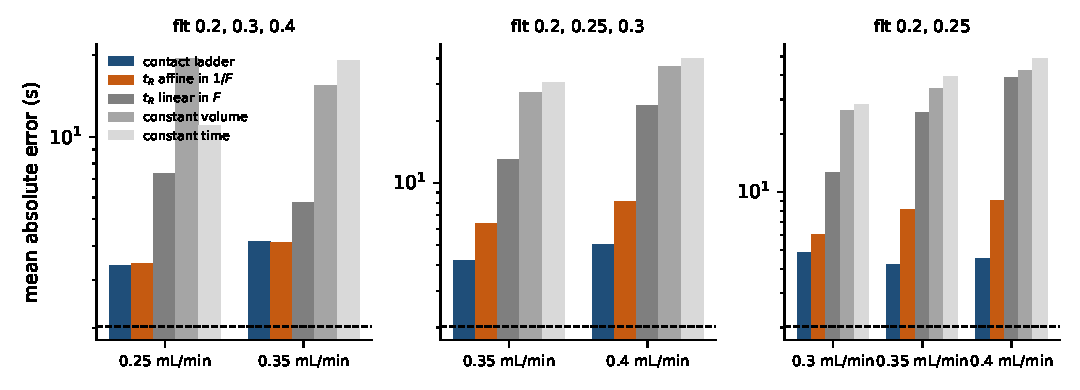
\includegraphics[width=\textwidth]{figures/fig1_flow.pdf}
\caption{Mean absolute error of retention time at held-out flow rates, on a logarithmic scale, for the three designs. The dashed line is the mean replicate difference between ionisation modes.}
\label{fig:flow}
\end{figure}

The advantage lies with retained compounds (Table~\ref{tab:split}).
About two thirds of the compounds had $k<1$ at the starting composition and eluted close to the dead time.
For the 124 or 125 compounds with $k>1$ at the start, the ladder error in the two extrapolation designs was 9.2 to 10.8\,s against 12.7 to 22.0\,s for the affine law.
For weakly retained compounds the affine law was slightly better in interpolation, 1.0 against 1.4\,s (Table~\ref{tab:split}).

\begin{table}[ht]
\centering
\caption{Mean absolute error (s) of the ladder model and of the affine law in $1/F$, separately for compounds with $k>1$ and $k\le1$ at the starting composition.}
\label{tab:split}
\begin{tabular}{@{}llrrrr@{}}
\toprule
 & & \multicolumn{2}{c}{$k>1$ (retained)} & \multicolumn{2}{c}{$k\le1$} \\
Design & Test & Ladder & Affine & Ladder & Affine \\
\midrule
Interpolation & 0.25 & 7.18 & 8.07 & 1.37 & 0.98 \\
              & 0.35 & 9.15 & 10.01 & 1.48 & 0.99 \\
Extrapolation & 0.35 & 9.20 & 14.26 & 1.59 & 2.19 \\
              & 0.40 & 10.77 & 18.47 & 2.03 & 2.64 \\
Two flows     & 0.30 & 9.93 & 12.75 & 2.18 & 2.45 \\
              & 0.35 & 9.41 & 19.92 & 1.47 & 1.91 \\
              & 0.40 & 9.40 & 22.03 & 1.95 & 2.28 \\
\bottomrule
\end{tabular}
\end{table}

The dwell volume selected was 0 to 0.1\,mL.
With two training flow rates the dwell volume is not identified by the data.
Fixing it anywhere between 0 and 0.2\,mL kept the two-flow errors between 4.1 and 5.8\,s, below the affine law in every case.
The median fitted solvent sensitivity was $S\approx10$.
Prediction~\ref{pr:flow} is supported.

\subsection{Elimination of the carrier}

Table~\ref{tab:carrier} and Figure~\ref{fig:carrier} compare the four groups of dataset pairs.
Under shared contacts but a different carrier, the median Spearman correlation of elution order was 0.995, against 0.997 for replicates.
A different stationary phase with the same mobile phase lowered it to 0.953, and a different organic modifier to 0.926.
The elution order is thus set by the contacts, and the carrier changes it little.
Prediction~\ref{pr:carrier} is supported.

\begin{table}[ht]
\centering
\caption{Agreement of elution compositions between pairs of datasets with at least twenty shared compounds.}
\label{tab:carrier}
\begin{tabular}{@{}lrrr@{}}
\toprule
Group & Pairs & Median Spearman $\rho$ & Median $|\Delta\varphi_e|$ \\
\midrule
Replicate & 172 & 0.997 & 0.005 \\
Same contacts, different carrier & 405 & 0.995 & 0.045 \\
Different column, same mobile phase & 2069 & 0.953 & 0.084 \\
Different organic modifier & 5090 & 0.926 & 0.162 \\
\bottomrule
\end{tabular}
\end{table}

\begin{figure}[ht]
\centering
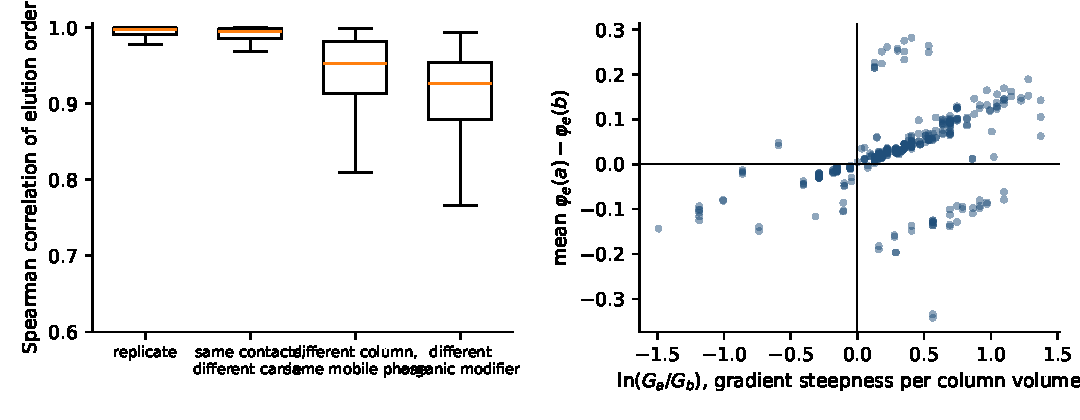
\includegraphics[width=\textwidth]{figures/fig2_contacts_carrier.pdf}
\caption{Left: Spearman correlation of elution order between pairs of datasets, by group. Right: for pairs with shared contacts, the mean difference in elution composition against the log-ratio of their gradient steepness per column volume.}
\label{fig:carrier}
\end{figure}

The absolute elution composition did shift between datasets with shared contacts, by a median of 0.045.
The shift followed the steepness of the program per column volume, with Spearman correlation 0.60 between the log-ratio of steepness and the mean shift ($p\approx4\times10^{-41}$).
The fitted slope, 0.076 per unit of log-ratio, corresponds by Corollary~\ref{cor:steepness} to a solvent sensitivity of about 13, close to the median of 10 fitted independently in the flow-rate series.
Removing the predicted shift, with the slope fitted on random halves of the pairs and applied to the other halves, reduced the median absolute shift from 0.044 to 0.012.
Prediction~\ref{pr:steepness} is supported.

After the mean shift of each pair was removed, the remaining disagreement had a median of 0.011 under shared contacts, against 0.004 for replicates.
In a regression of this remainder on the carrier differences, the steepness term was positive with a 95\% confidence interval of 0.009 to 0.041.
The terms for column length, diameter and flow rate had intervals that contained zero.
The particle-size term had a point estimate of 0.10 and an interval from 0 to 0.82, so an effect of particle size is neither established nor excluded by these data.

\subsection{Transfer through the hydrophobic-subtraction parameters}

Prediction~\ref{pr:hsm} is not supported (Figure~\ref{fig:hsm}).
For acetonitrile, the column-agnostic elution order reached a mean Spearman correlation of 0.868 on held-out columns, the order predicted from the five parameters 0.867, and the oracle 0.937.
For methanol the corresponding values were 0.837, 0.833 and 0.917.
The gap between the column-agnostic order and the oracle shows that each column has a column-specific elution order (Figure~\ref{fig:hsm}, left).
The five parameters did not predict it: the mean correlation of the predicted and observed column-specific parts, averaged per column, was $-0.10$ for acetonitrile and $0.00$ for methanol, with one-sided Wilcoxon $p$-values of 0.84 and 0.51.
In the inverse direction, none of the five parameters was recovered from retention data: every cross-validated coefficient of determination was negative, and the smallest permutation $p$-value was 0.19.
Across pairs of different columns, the distance between their parameter vectors correlated with the disagreement in elution order with Spearman correlation 0.37, but a permutation test of the columns gave $p=0.08$.

\begin{figure}[ht]
\centering
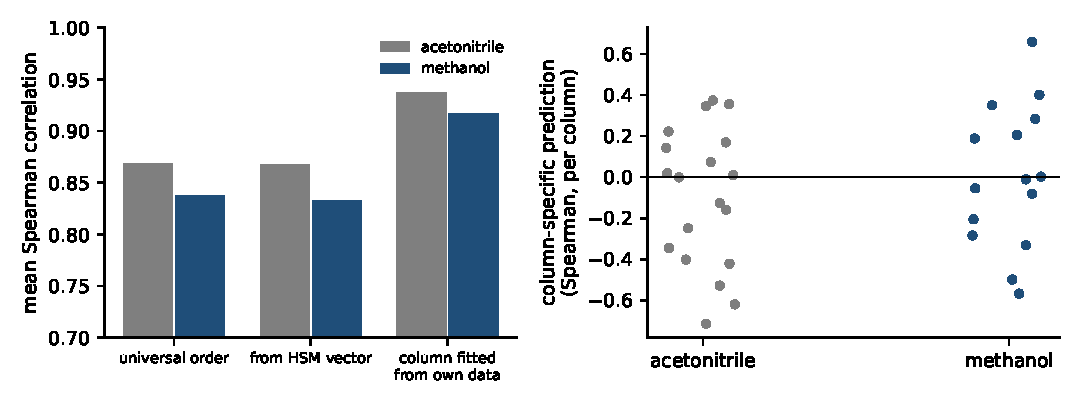
\includegraphics[width=\textwidth]{figures/fig3_hsm.pdf}
\caption{Left: mean Spearman correlation of predicted and observed elution order on held-out columns, for a column-agnostic order, an order predicted from the hydrophobic-subtraction parameters, and an oracle. Right: correlation between predicted and observed column-specific order, one point per held-out column.}
\label{fig:hsm}
\end{figure}

\subsection{Richer contact descriptions}

Table~\ref{tab:rich} and Figure~\ref{fig:rich} give the results of the exploratory analysis of Section~\ref{sec:rich-methods}.
Adding nine stationary-phase numbers to the five did not help.
With 14 numbers, no model predicted the column-specific order on a held-out column for either modifier (Table~\ref{tab:rich}, rows 2 and 6).
In Model~A, the largest ridge strength offered was selected in 94--100\% of the folds for every description but one, so the cross-validation preferred to shrink the map towards zero.
The exception was the eluent description for methanol, with 57\%.

The eluent numbers carried a signal.
For methanol, on held-out columns, the eluent description gave a mean column-specific correlation of 0.25 in Model~B (Table~\ref{tab:rich}, row 7).
The predicted direction was correct for 82\% of the held-out datasets.
Model~A gave 0.28 with the same description.
When whole laboratories were held out, the eluent description still predicted the specific order for both modifiers.
The means were 0.18 for acetonitrile and 0.32 for methanol, both with $p<10^{-4}$ (Table~\ref{tab:rich}, rows 3 and 7).
Of the eluent numbers, the additive indicators carried more of the signal than the pH (Figure~\ref{fig:rich}, right).

The eluent prediction had the right direction but not the right size.
The overall elution order it predicted on held-out columns was no better than the column-agnostic order (Table~
ef{tab:rich}, caption).
The column-specific part is small compared with the shared order, and the fitted responses over-shot it.

The five HSM numbers also scored well when laboratories were held out (0.33 and 0.28; Figure~\ref{fig:rich}, right).
That score does not measure transfer to an unseen phase, because the column of a held-out laboratory was used by another laboratory in 49 of 85 acetonitrile datasets and 41 of 92 methanol datasets.

The two similarity tests were weak.
For acetonitrile, the training dataset nearest in the five HSM numbers agreed with the held-out order better than an average training dataset.
The advantage was 0.019 in Spearman correlation, with a permutation $p$-value of 0.017.
For methanol the advantage was 0.042, with $p=0.06$.
With the 14 column numbers neither advantage was significant ($p=0.15$ and $0.24$).
Kernel-weighted transfer was worse than the column-agnostic order for both modifiers.

\begin{table}[ht]
\centering
\caption{Prediction of the column-specific elution order from contact descriptions of increasing size (Model~B). Each entry is the mean, over held-out columns or laboratories, of the Spearman correlation between predicted and observed column-specific order, with the one-sided Wilcoxon $p$-value. A dash marks a combination that was not run. On held-out columns, the overall elution order predicted from the eluent description had a mean Spearman correlation of 0.926 (acetonitrile) and 0.910 (methanol), against 0.941 and 0.902 for the column-agnostic order.}
\label{tab:rich}
\begin{tabular}{llcccc}
\toprule
 & & \multicolumn{2}{c}{held-out column} & \multicolumn{2}{c}{held-out laboratory} \\
\cmidrule(lr){3-4}\cmidrule(lr){5-6}
Modifier & Description & mean & $p$ & mean & $p$ \\
\midrule
Acetonitrile & HSM (5) & $-0.01$ & 0.66 & 0.33 & $<10^{-6}$ \\
 & Column (14) & $-0.04$ & 0.80 & -- & -- \\
 & Eluent (9) & 0.04 & 0.08 & 0.18 & $<10^{-5}$ \\
 & All (23) & $-0.01$ & 0.62 & 0.50 & $<10^{-9}$ \\
Methanol & HSM (5) & 0.13 & 0.03 & 0.28 & $<10^{-3}$ \\
 & Column (14) & 0.07 & 0.18 & -- & -- \\
 & Eluent (9) & 0.25 & $<10^{-3}$ & 0.32 & $<10^{-4}$ \\
 & All (23) & 0.24 & $<10^{-3}$ & 0.40 & $<10^{-4}$ \\
\bottomrule
\end{tabular}
\end{table}

\begin{figure}[ht]
\centering
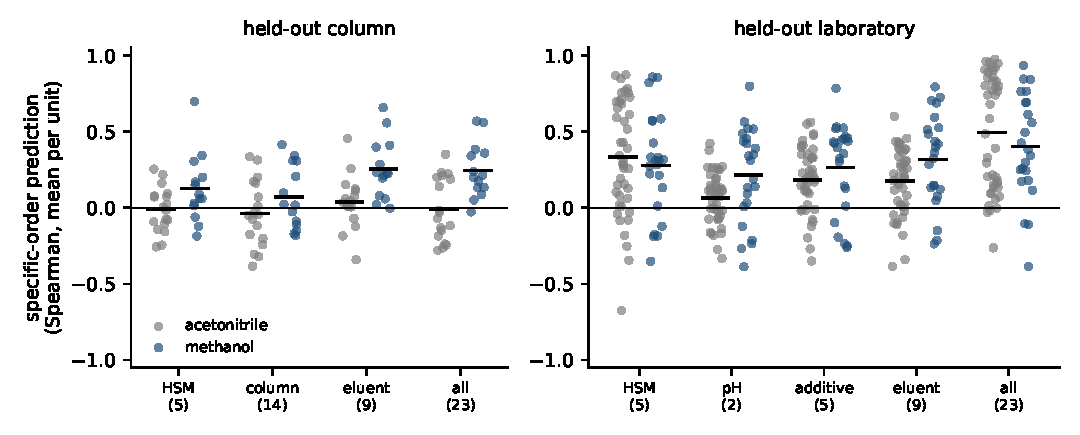
\includegraphics[width=\textwidth]{figures/fig4_contacts.pdf}
\caption{Prediction of the column-specific elution order from contact descriptions (Model~B); the number of contact numbers is in parentheses. Each point is one held-out column (left) or one held-out laboratory (right), and bars mark means.}
\label{fig:rich}
\end{figure}

%======================================================================
\section{Discussion}
\label{sec:discussion}
%======================================================================

\subsection{What the tests support}

Three of the four predictions held.
Retention on one column at five flow rates was described by two numbers per compound and one dwell volume, with errors near the replicate noise and below those of empirical flow laws in extrapolation.
Across 290 datasets from many laboratories, the elution order under shared contacts was as stable as between replicates, whatever the column dimensions, particle size, flow rate or program.
The absolute elution composition moved with the gradient steepness per column volume, in the direction and with the magnitude of Corollary~\ref{cor:steepness}.
Two independent estimates of the solvent sensitivity, from the flow series and from the steepness shift across laboratories, agreed to within a factor of 1.3.

The three supported predictions bear out the central claim of the ladder description: once the contacts and their schedule are fixed, the carrier adds little to the readout.
The dwell volume and the gradient steepness are not removed by the elimination, and Remark~\ref{rem:dwell} explains why: they change when each contact occurs.
An unreported dwell volume is the likeliest source of the remaining disagreement under shared contacts, which was 2.8 times the replicate level.

\subsection{What the tests do not support}

The fourth prediction failed.
Five numbers per stationary phase did not carry the column-specific part of the elution order to an unseen column, and could not be recovered from retention.
The exploratory analysis separates two of the possible reasons.
The dataset factors combine the stationary phase with the eluent, which the column parameters do not describe.
When the eluent was described, its contacts carried the specific order to new columns for methanol and to new laboratories for both modifiers (Table~\ref{tab:rich}).
Ammonium salts or basic additives were used in 16 of 92 methanol datasets but only 8 of 85 acetonitrile datasets.
Its larger eluent effect is consistent with the ionisation of the analytes, which those additives control.
Adding stationary-phase numbers did not help.
The Tanaka and HSM parameters are measured with a few neutral test solutes at fixed conditions \citep{snyder2004,kimata1989}, while the compounds here are metabolites, many of them ionisable.
With 14 to 18 columns per modifier, the maps from 14 numbers are also estimated from few points.

For the design of separations by their contacts, the consequence is specific.
The carrier can be set aside (Tables~\ref{tab:flow} and~\ref{tab:carrier}), so a separation is described by the contacts of each analyte with each stationary phase and mobile phase.
The mobile-phase contacts transfer between laboratories through a handful of numbers, which makes changing the eluent a change of contacts in the sense intended.
The stationary-phase contacts are not summarised by tabulated test-solute parameters for analytes of this kind.
Calculating a stationary phase backwards from a desired ladder therefore needs contact numbers measured with analytes that resemble the targets, under the eluent that will be used.

\subsection{Limitations}

The repository contains almost no isocratic data, so Theorem~\ref{thm:isocratic} was not tested directly.
Peak widths are not reported, so band broadening was not tested.
Dwell volumes are not reported and were set to zero outside the flow-rate series.
In datasets 0310--0341 the column named in the metadata and the column named in the dataset label differ for two columns.
Neither column has hydrophobic-subtraction parameters, so the transfer test is unaffected, but the grouping of those datasets in the carrier test depends on which label is correct.
The gradient equations coincide with an established model \citep{snyder2007}, so the agreement with data in the first test is also evidence for that model.
The ladder description contributes the elimination statement and its tests.

\section{Conclusion}
\label{sec:conclusion}

Liquid chromatography can be written as a contact ladder.
An analyte's elution is fixed by its stays in the stationary phase and by the schedule on which they occur, and the column bed, geometry and flow can be removed from the description.
The gradient form of the ladder has an exact solution for a linear program that contains no column dimension or flow rate.
On public data the description predicted retention across flow rates, kept the elution order fixed across laboratories with shared contacts, and predicted the effect of gradient steepness.
It did not allow retention to be transferred between stationary phases through their five hydrophobic-subtraction parameters, nor through 14 tabulated column parameters.
Nine numbers describing the eluent did carry the direction of the column-specific order to new laboratories.
The open problem is therefore the description of the stationary-phase contacts.

\section*{Data and code availability}
\addcontentsline{toc}{section}{Data and code availability}
The data are from RepoRT \citep{kretschmer2024}, commit \texttt{420b550}, under the Creative Commons Attribution--ShareAlike 4.0 licence.
The analysis scripts are in the directory \texttt{examples/\allowbreak chromatography/\allowbreak contact\_ladder\_validation} of the repository that contains this manuscript.

\bibliographystyle{unsrtnat}
\bibliography{references}

\end{document}
